The Internet of Things (IoT) is a rapidly emerging set of technologies in which ordinary objects are equipped with digital intelligence -- the ability to sense, analyze, and control their environment automatically. By linking the physical and digital worlds, IoT has the potential to enhance situational awareness and effective decision-making by humans, to detect, diagnose, and remediate problems without human intervention, to assist with personal and homeland security, to optimize manufacturing and business processes, and to automate operations throughout the economy.

To realize this impact, IoT must be embedded in the world around us -- within buildings, cars, roads, homes, industrial machinery, and waterways, and distributed across farms, wild open spaces, cities, and oceans. Moreover, they increasingly leverage recent advances in data analytics, machine learning (ML), and automation \textit{in-situ} -- at the edge of the network -- ``near'' (in terms of network latency) the locus of sensing and/or actuation. This move to the edge is the result of an increase in the velocity and volume of data and high response latencies imposed by the long-haul, intermittently available networks that connect the edge and cloud. Further, unlike in the context of e-commerce and other cloud application domains, IoT applications often benefit from spatial locality in terms of performance, robustness, and security. That is, co-location of processing infrastructure and IoT devices significantly reduces the latency between data acquisition and device actuation, enables extension of device capability via local offloading, and alleviates the cost, power consumption, and congestion of network use versus the centralized, cloud-direct model~\cite{edge,bonomi2012fog,cloudlets,cloudlets2012satya,verbelen2012cloudlets}.

Edge processing, however, introduces new challenges for IoT deployments. Unlike the devices themselves, edge computing elements are often designed for environments in which the ambient environmental conditions are controlled and kept within a narrow operational range. The operational settings in which these edge systems (in our work we deploy miniturized ``edge clouds'' using clusters of commodity small-board computers to support IoT analytics) are deployed can be harsh, hard or costly to access, and exposed to harmful environmental elements (heat, moisture, dust, animals, other objects, humans, weather, etc.). For example, we currently support an IoT deployment for image processing and deep learning for the automatic, real time identification of animals using camera traps deployed across UCSB Sedgwick Reserve, an ecology and wildlife educational and research reserve in California~\cite{ref:sedgwick}. The reserve is 6,000 acres that comprises critical wildlife habitats, two watersheds at the foot of Figueroa Mountain in Santa Ynez, California, and a 300-acre farm easement. Our edge clouds fuse and analyze images from within out-buildings on the property. Sedgwick yearly outdoor temperatures range between 30$^{\circ}$ and 116$^{\circ}$ Fahrenheit; within enclosures (e.g. shelters for electrical pumping equipment where grid electricity is available) our cloud systems are subjected to much higher ambient operating temperatures.

Excessive heat can degrade the performance and reliability of devices and negatively impact their longevity (requiring more human intervention and frequent replacement). Commodity computers are particularly sensitive to high temperatures and extended exposure can cause these machines to break down, degrade in functionality, and fail prematurely -- even they are protected using operational safeguards such as throttling and automatic shutdown~\cite{ref:overheating}. For this reason, most manufacturers include an on-board thermal CPU temperature sensor and the ability to set a ``shut-down'' temperature if the CPU exceeds the manufacturer's maximum supported temperature. Figure\ref{fig:time_series} shows a time series of CPU temperature in degrees Fahrenheit gathered from one of our edge clouds deployed at Sedgwick between February, 2018 and and June, 2020. The cut-off temperatures was set to 200\degree F and the temperature drop early in the trace records the system's automatic shutdown.

\begin{figure}
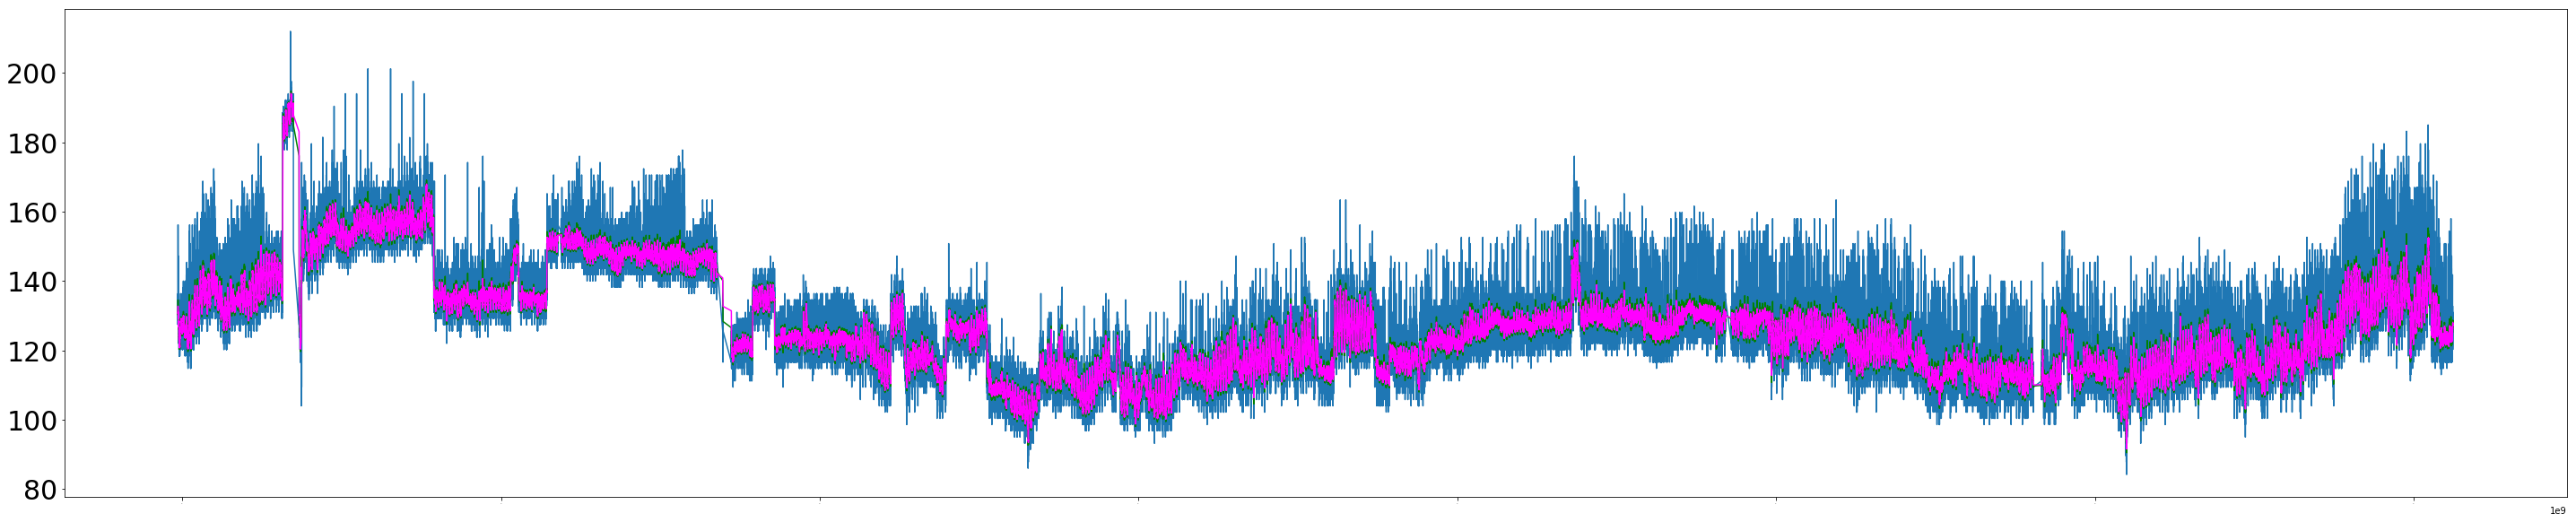
\includegraphics[width=\textwidth]{figures/time_series.png}
\caption{The time series of CPU temperature in the edge cloud deployed at Sedgwick Natural Reserve from Feb. 28th, 2018 to Jun. 3rd, 2020. The x-axis is the epoch time and the y-axis is the CPU temperature in Fahrenheit. } \label{fig:time_series}
\end{figure}

In this paper, we investigate the use of dynamic voltage and frequency scaling (DVFS)~\cite{ref:Liu2007dvfs,ref:Wang2010dvfs,ref:Wu2013dvfs} to control system temperature when the ambient temperature might cause it to exceed the acceptable operational range. DVFS is a technique that has been widely studied in the context of ``power capping'' -- the implementation of a maximum power draw by the system.  Our system -- called \textit{Sparta} --  automatically exploits the relationship between system power consumption and generated heat.  It does so by adjusting processor frequency dynamically so that CPU temperatures do not exceed a specified threshold as ambient temperature changes.  Subject to the threshold, the system attempts to minimize the application ``slow down'' (relative to maximum CPU frequency) that frequency adjustments might introduce.  
We use Sparta to study the relationships between CPU frequency, temperature, power dissipation, and execution behavior. Moreover, we consider IoT workloads that employ a wide range of machine learning algorithms, including image recognition, natural language processing, decision forest and time series prediction. 

%Sparta takes an application, corresponding dataset and a configurable temperature threshold as inputs and automatically schedules the workload based on the online sampling temperature data. We use the system to perform a 
%range of machine learning algorithms, including image recognition, natural language processing, decision forest and time series prediction. This benchmark suite represents different execution patterns in machine learning applications that we utilize in the real-world IoT settings. 

We consider three modes for the Sparta frequency scheduler: \textbf{Annealing}, \textbf{AIMD}, and \textbf{Hybrid}.  Annealing employs an epsilon-greedy strategy to extrapolate an appropriate CPU frequency in real time. AIMD uses the linear growth of CPU frequency when temperature is under threshold and exponential reduction when it detects temperature anomalies to determine its CPU frequency.  With Hybrid, we combine the best features of the two modes to overcome their drawbacks. Our results show that Sparta in Hybrid mode speeds up the execution of our applications by \textbf{1.16x} and \textbf{1.14x} on average in three thermal environments compared to Annealing and AIMD. Moreover, Sparta in Hybrid mode maintains CPU temperature below threshold \textbf{94.4\%} of the time (as measured via temperature sampling), on average across all benchmarks. 

In summary, with this paper, we make the following contributions:
\begin{itemize}
    \item We investigate the relationship between CPU frequency and sampling temperature to precisely model and manage processor power dissipation during execution;
    \vspace{1mm}
    \item We design and implement a heat-budget-based scheduling framework that protects edge systems from overheating and potential damage;
    \vspace{1mm}
    \item We empirically evaluate the efficacy of using Sparta to control CPU temperature and accelerate machine learning applications on six real-world benchmarks in three thermal deployment environments. 
\end{itemize}

In the following sections, we present the design and implementation of Sparta (Section~\ref{sec:Sparta}). We then describe our experimental methodology and empirical evaluation of the system using multiple machine learning applications in different thermal environments (Section~\ref{sec:eval}). In Section~\ref{sec:relate_work},  we discuss related work. Finally, we present our conclusions and future work plans.



\ignore{
Cloud computing enables the delivery of numerous computing services, including processing power, data storage, data analytics, networking and software, over the Internet. The demand on scalable and agile services has triggered an ecosystem of cloud computing, in which users can optimize cloud systems by integrating virtualized resources and obtain cost advantage compared to in-house IT infrastructure. In addition, the autoscaling of elastic services automatically allocate computational resources when the production workloads are unpredictable, allowing the system to handle the variable traffic spikes better.

To address the security concern and networking latency, cloud computing has evolved into a stratified system that contains IoT clusters, edge cloud and data centers. In this paradigm, edge cloud serves as the middle layer between IoT devices and data centers that brings the computational power and data storage near the deployment sites in hope of improving round-trip time and bandwidth usage. Thus, in the scenarios like real-time data streaming from sensors or users, edge cloud plays a critical role in timely execution and content delivery. 

Particularly, with the arrival of powerful edge cloud devices, computing tasks that requires significant computational power can now be executed on edge devices. Such capability brings more complex machine learning models that analyzes large amounts of dataset closer to data sources and reduces networking latency. This movement has given rise to "edge-based" machine learning that deploys advanced algorithms such as convolutional neural networks (CNNs) at the edge of the network.
}
